% Options for packages loaded elsewhere
\PassOptionsToPackage{unicode}{hyperref}
\PassOptionsToPackage{hyphens}{url}
%
\documentclass[
  12pt,
]{article}
\usepackage{lmodern}
\usepackage{amsmath}
\usepackage{ifxetex,ifluatex}
\ifnum 0\ifxetex 1\fi\ifluatex 1\fi=0 % if pdftex
  \usepackage[T1]{fontenc}
  \usepackage[utf8]{inputenc}
  \usepackage{textcomp} % provide euro and other symbols
  \usepackage{amssymb}
\else % if luatex or xetex
  \usepackage{unicode-math}
  \defaultfontfeatures{Scale=MatchLowercase}
  \defaultfontfeatures[\rmfamily]{Ligatures=TeX,Scale=1}
  \setmainfont[]{Times New Roman}
\fi
% Use upquote if available, for straight quotes in verbatim environments
\IfFileExists{upquote.sty}{\usepackage{upquote}}{}
\IfFileExists{microtype.sty}{% use microtype if available
  \usepackage[]{microtype}
  \UseMicrotypeSet[protrusion]{basicmath} % disable protrusion for tt fonts
}{}
\makeatletter
\@ifundefined{KOMAClassName}{% if non-KOMA class
  \IfFileExists{parskip.sty}{%
    \usepackage{parskip}
  }{% else
    \setlength{\parindent}{0pt}
    \setlength{\parskip}{6pt plus 2pt minus 1pt}}
}{% if KOMA class
  \KOMAoptions{parskip=half}}
\makeatother
\usepackage{xcolor}
\IfFileExists{xurl.sty}{\usepackage{xurl}}{} % add URL line breaks if available
\IfFileExists{bookmark.sty}{\usepackage{bookmark}}{\usepackage{hyperref}}
\hypersetup{
  pdftitle={Evaluation of Water Quality in Eno River and Ellerbe Creek in 2019 and 2020},
  pdfauthor={Olivia August and Analise Lindborg},
  hidelinks,
  pdfcreator={LaTeX via pandoc}}
\urlstyle{same} % disable monospaced font for URLs
\usepackage[margin=2.54cm]{geometry}
\usepackage{longtable,booktabs}
\usepackage{calc} % for calculating minipage widths
% Correct order of tables after \paragraph or \subparagraph
\usepackage{etoolbox}
\makeatletter
\patchcmd\longtable{\par}{\if@noskipsec\mbox{}\fi\par}{}{}
\makeatother
% Allow footnotes in longtable head/foot
\IfFileExists{footnotehyper.sty}{\usepackage{footnotehyper}}{\usepackage{footnote}}
\makesavenoteenv{longtable}
\usepackage{graphicx}
\makeatletter
\def\maxwidth{\ifdim\Gin@nat@width>\linewidth\linewidth\else\Gin@nat@width\fi}
\def\maxheight{\ifdim\Gin@nat@height>\textheight\textheight\else\Gin@nat@height\fi}
\makeatother
% Scale images if necessary, so that they will not overflow the page
% margins by default, and it is still possible to overwrite the defaults
% using explicit options in \includegraphics[width, height, ...]{}
\setkeys{Gin}{width=\maxwidth,height=\maxheight,keepaspectratio}
% Set default figure placement to htbp
\makeatletter
\def\fps@figure{htbp}
\makeatother
\setlength{\emergencystretch}{3em} % prevent overfull lines
\providecommand{\tightlist}{%
  \setlength{\itemsep}{0pt}\setlength{\parskip}{0pt}}
\setcounter{secnumdepth}{5}
\ifluatex
  \usepackage{selnolig}  % disable illegal ligatures
\fi

\title{Evaluation of Water Quality in Eno River and Ellerbe Creek in
2019 and 2020}
\usepackage{etoolbox}
\makeatletter
\providecommand{\subtitle}[1]{% add subtitle to \maketitle
  \apptocmd{\@title}{\par {\large #1 \par}}{}{}
}
\makeatother
\subtitle{\url{https://github.com/arl57/EDA_Final_Project_DurhamWQ}}
\author{Olivia August and Analise Lindborg}
\date{}

\begin{document}
\maketitle

\newpage
\tableofcontents 
\newpage
\listoftables 
\newpage
\listoffigures 
\newpage

\hypertarget{rationale-and-research-questions}{%
\section{Rationale and Research
Questions}\label{rationale-and-research-questions}}

Water quality of urban streams and rivers has been studied across the
United States for the past several decades. These evaluations typically
provide important insights about stressors on aquatic systems in urban
environments, particularly natural pollutants such as nutrients,
sediment, and heavy metals, as well as anthropogenic contaminants such
as pesticides and other man-made chemicals. Many cities have programs
dedicated to monitoring the health of local rivers and streams for the
protection of humans and wildlife.

Certain water quality parameters are commonly collected and used to
assess health of urban streams. These include measurements of chemical,
physical, and biological parameters that can be used independently or
together to determine stream health. These parameters are often
evaluated over time to highlight general trends in water quality in
urban environments. In general, health of urban streams in the United
States has been improving since the Clean Water Act was introduced in
the 1970s.

The main objective of our project was to understand current water
quality trends in local urban streams between 2019 and 2020. Eno River
and Ellerbe Creek in Durham, North Carolina were selected for evaluation
in our study. These streams were chosen to provide a local context for
evaluating recent changes in stream health. Additionally, the City of
Durham collects monthly monitoring data for both Eno River and Ellerbe
Creek for several metrics that they provide publicly, making this easily
accessible data. This project includes an evaluation of the most common
surface water quality parameters for which the City of Durham had data,
including temperature, pH, dissolved oxygen, metals (zinc and copper),
total phosphorus, fecal coliform, turbidity, and total suspended solids.
All sites for each water body evaluated by the City of Durham were
included.

\textbf{Research Question:}

\begin{enumerate}
\def\labelenumi{\arabic{enumi}.}
\tightlist
\item
  What are the water quality trends between 2019 and 2020 for Ellerbe
  Creek and Eno River?

  \begin{enumerate}
  \def\labelenumii{\alph{enumii}.}
  \tightlist
  \item
    Has water quality changed between 2019 and 2020 for Ellerbe Creek
    and/or Eno River based on the various water quality parameters?
  \item
    Have certain water quality parameters changed while others have not?
  \end{enumerate}
\end{enumerate}

\hypertarget{dataset-information}{%
\section{Dataset Information}\label{dataset-information}}

The data was collected from the City of Durham's water quality data web
portal. The portal includes data collected by the City's Stormwater
Services as part of the Water Quality Monitoring and Assessment Program.
The program performs ambient stream monitoring to assess compliance with
regulatory benchmarks, assess surface water impairment, identify sources
for illicit discharge, and support watershed planning. The monitoring
data includes information regarding the monitoring location, conditions,
weather, and measurements. Nine parameters were chosen for analysis
because of their monthly measurement frequency for 2019 and 2020 at the
two streams of interest. The parameters of interest include Copper,
Dissolved Oxygen, Fecal Coliform, pH, Total Phosphorus, Total Suspended
Solids, Temperature, Turbidity, and Zinc. To extract relevant data from
the portal the stream, water quality parameters, and dates of interest
were selected for the user interface and downloaded to CSV files.

Once datasets for each of the parameters were downloaded, they were read
into R and compiled into a single dataframe. First, a subset of the
dataframe was created to keep only relevant columns for analysis. Next,
the date column to read as a date to enable plotting and time series
analysis. To address duplicate measurements, measurements for the same
parameter, with the same date and monitoring location were averaged.
Then, the parameters measurements were pivoted to include a column for
each of the nine parameters. To map the locations of each of the
monitoring stations, the water quality dataframe was joined with station
coordinates.

\begin{longtable}[]{@{}llll@{}}
\toprule
\begin{minipage}[b]{(\columnwidth - 3\tabcolsep) * \real{0.49}}\raggedright
Water Quality Parameters\strut
\end{minipage} &
\begin{minipage}[b]{(\columnwidth - 3\tabcolsep) * \real{0.12}}\raggedright
Unit\strut
\end{minipage} &
\begin{minipage}[b]{(\columnwidth - 3\tabcolsep) * \real{0.14}}\raggedright
Range\strut
\end{minipage} &
\begin{minipage}[b]{(\columnwidth - 3\tabcolsep) * \real{0.25}}\raggedright
Data Source\strut
\end{minipage}\tabularnewline
\midrule
\endhead
\begin{minipage}[t]{(\columnwidth - 3\tabcolsep) * \real{0.49}}\raggedright
Copper\strut
\end{minipage} &
\begin{minipage}[t]{(\columnwidth - 3\tabcolsep) * \real{0.12}}\raggedright
ug/L\strut
\end{minipage} &
\begin{minipage}[t]{(\columnwidth - 3\tabcolsep) * \real{0.14}}\raggedright
1.1-4.135\strut
\end{minipage} &
\begin{minipage}[t]{(\columnwidth - 3\tabcolsep) * \real{0.25}}\raggedright
Durham Water Quality Web Portal\strut
\end{minipage}\tabularnewline
\begin{minipage}[t]{(\columnwidth - 3\tabcolsep) * \real{0.49}}\raggedright
Dissolved Oxygen\strut
\end{minipage} &
\begin{minipage}[t]{(\columnwidth - 3\tabcolsep) * \real{0.12}}\raggedright
mg/L\strut
\end{minipage} &
\begin{minipage}[t]{(\columnwidth - 3\tabcolsep) * \real{0.14}}\raggedright
4.7-12.1\strut
\end{minipage} &
\begin{minipage}[t]{(\columnwidth - 3\tabcolsep) * \real{0.25}}\raggedright
Durham Water Quality Web Portal\strut
\end{minipage}\tabularnewline
\begin{minipage}[t]{(\columnwidth - 3\tabcolsep) * \real{0.49}}\raggedright
Fecal Coliform\strut
\end{minipage} &
\begin{minipage}[t]{(\columnwidth - 3\tabcolsep) * \real{0.12}}\raggedright
cfu/100mL\strut
\end{minipage} &
\begin{minipage}[t]{(\columnwidth - 3\tabcolsep) * \real{0.14}}\raggedright
17.5-36000\strut
\end{minipage} &
\begin{minipage}[t]{(\columnwidth - 3\tabcolsep) * \real{0.25}}\raggedright
Durham Water Quality Web Portal\strut
\end{minipage}\tabularnewline
\begin{minipage}[t]{(\columnwidth - 3\tabcolsep) * \real{0.49}}\raggedright
pH\strut
\end{minipage} &
\begin{minipage}[t]{(\columnwidth - 3\tabcolsep) * \real{0.12}}\raggedright
Standard Units\strut
\end{minipage} &
\begin{minipage}[t]{(\columnwidth - 3\tabcolsep) * \real{0.14}}\raggedright
6.1-7.5\strut
\end{minipage} &
\begin{minipage}[t]{(\columnwidth - 3\tabcolsep) * \real{0.25}}\raggedright
Durham Water Quality Web Portal\strut
\end{minipage}\tabularnewline
\begin{minipage}[t]{(\columnwidth - 3\tabcolsep) * \real{0.49}}\raggedright
Total Phosphorus\strut
\end{minipage} &
\begin{minipage}[t]{(\columnwidth - 3\tabcolsep) * \real{0.12}}\raggedright
mg/L\strut
\end{minipage} &
\begin{minipage}[t]{(\columnwidth - 3\tabcolsep) * \real{0.14}}\raggedright
0.003 - 0.38\strut
\end{minipage} &
\begin{minipage}[t]{(\columnwidth - 3\tabcolsep) * \real{0.25}}\raggedright
Durham Water Quality Web Portal\strut
\end{minipage}\tabularnewline
\begin{minipage}[t]{(\columnwidth - 3\tabcolsep) * \real{0.49}}\raggedright
Total Suspended Solids\strut
\end{minipage} &
\begin{minipage}[t]{(\columnwidth - 3\tabcolsep) * \real{0.12}}\raggedright
mg/L\strut
\end{minipage} &
\begin{minipage}[t]{(\columnwidth - 3\tabcolsep) * \real{0.14}}\raggedright
2.5-134\strut
\end{minipage} &
\begin{minipage}[t]{(\columnwidth - 3\tabcolsep) * \real{0.25}}\raggedright
Durham Water Quality Web Portal\strut
\end{minipage}\tabularnewline
\begin{minipage}[t]{(\columnwidth - 3\tabcolsep) * \real{0.49}}\raggedright
Temperature\strut
\end{minipage} &
\begin{minipage}[t]{(\columnwidth - 3\tabcolsep) * \real{0.12}}\raggedright
C\strut
\end{minipage} &
\begin{minipage}[t]{(\columnwidth - 3\tabcolsep) * \real{0.14}}\raggedright
5.7-29.6\strut
\end{minipage} &
\begin{minipage}[t]{(\columnwidth - 3\tabcolsep) * \real{0.25}}\raggedright
Durham Water Quality Web Portal\strut
\end{minipage}\tabularnewline
\begin{minipage}[t]{(\columnwidth - 3\tabcolsep) * \real{0.49}}\raggedright
Turbidity\strut
\end{minipage} &
\begin{minipage}[t]{(\columnwidth - 3\tabcolsep) * \real{0.12}}\raggedright
NTU\strut
\end{minipage} &
\begin{minipage}[t]{(\columnwidth - 3\tabcolsep) * \real{0.14}}\raggedright
2.3-150\strut
\end{minipage} &
\begin{minipage}[t]{(\columnwidth - 3\tabcolsep) * \real{0.25}}\raggedright
Durham Water Quality Web Portal\strut
\end{minipage}\tabularnewline
\begin{minipage}[t]{(\columnwidth - 3\tabcolsep) * \real{0.49}}\raggedright
Zinc\strut
\end{minipage} &
\begin{minipage}[t]{(\columnwidth - 3\tabcolsep) * \real{0.12}}\raggedright
ug/L\strut
\end{minipage} &
\begin{minipage}[t]{(\columnwidth - 3\tabcolsep) * \real{0.14}}\raggedright
0.975-19.2\strut
\end{minipage} &
\begin{minipage}[t]{(\columnwidth - 3\tabcolsep) * \real{0.25}}\raggedright
Durham Water Quality Web Portal\strut
\end{minipage}\tabularnewline
\begin{minipage}[t]{(\columnwidth - 3\tabcolsep) * \real{0.49}}\raggedright
Rain in the last 24 Hours\strut
\end{minipage} &
\begin{minipage}[t]{(\columnwidth - 3\tabcolsep) * \real{0.12}}\raggedright
NA\strut
\end{minipage} &
\begin{minipage}[t]{(\columnwidth - 3\tabcolsep) * \real{0.14}}\raggedright
Yes/No\strut
\end{minipage} &
\begin{minipage}[t]{(\columnwidth - 3\tabcolsep) * \real{0.25}}\raggedright
Durham Water Quality Web Portal\strut
\end{minipage}\tabularnewline
\begin{minipage}[t]{(\columnwidth - 3\tabcolsep) * \real{0.49}}\raggedright
Sky Condition\strut
\end{minipage} &
\begin{minipage}[t]{(\columnwidth - 3\tabcolsep) * \real{0.12}}\raggedright
NA\strut
\end{minipage} &
\begin{minipage}[t]{(\columnwidth - 3\tabcolsep) * \real{0.14}}\raggedright
Sunny, Partly Cloudy, Overcast\strut
\end{minipage} &
\begin{minipage}[t]{(\columnwidth - 3\tabcolsep) * \real{0.25}}\raggedright
Durham Water Quality Web Portal\strut
\end{minipage}\tabularnewline
\bottomrule
\end{longtable}

\hypertarget{exploratory-analysis}{%
\section{Exploratory Analysis}\label{exploratory-analysis}}

As part of the exploratory analysis, water quality data was compiled for
the nine parameters for both the Eno River and Ellerbe Creek. The
following sections describe the exploratory analysis completed for each
waterway.

Both Ellerbe Creek and Eno River have three monitoring stations in
Durham. Sites EN13.3ER, EN8.9ER, and EN4.9ER for Eno River all had data
for 2020, but only EN8.9ER had data for 2019. For Ellerbe Creek, sites
EL1.9EC, EL5.6EC, and EL7.1EC had data for 2019, but only EL1.9EC and
EL7.1EC had data for 2020.

\begin{figure}

{\centering 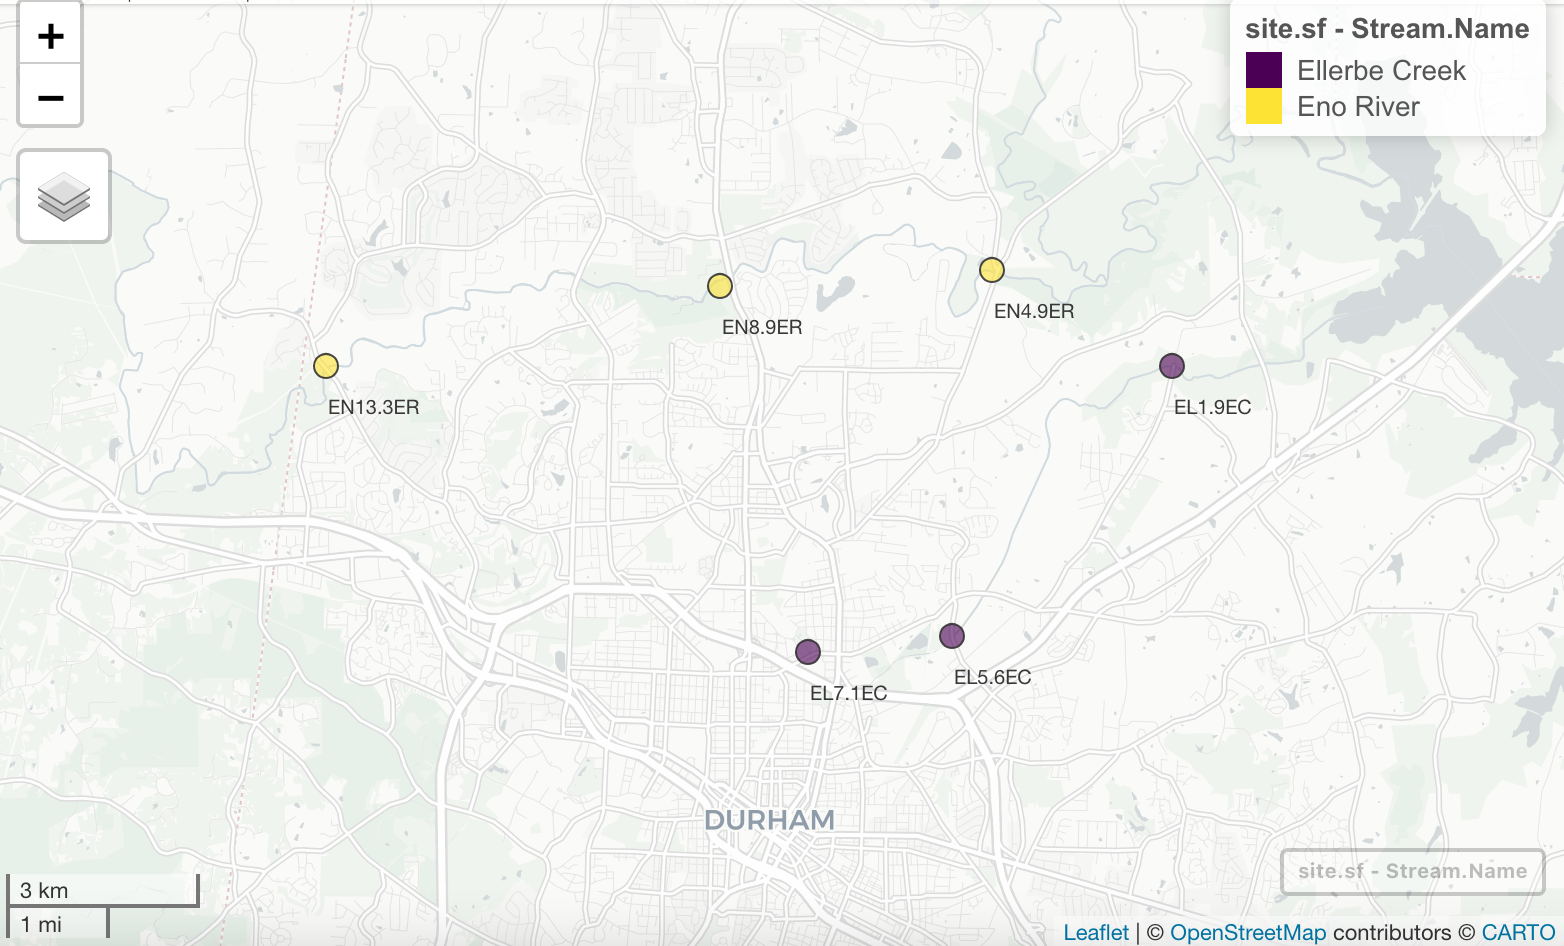
\includegraphics[width=1\linewidth]{Output/SiteMap} 

}

\caption{Site Map of Ellerbe Creek and Eno River Monitoring Stations}\label{fig:unnamed-chunk-1}
\end{figure}

\hypertarget{eno-river}{%
\subsection{Eno River}\label{eno-river}}

The first part of the analysis included a comparative visualization of
the nine water quality parameters for 2019 and 2020. In order to get a
better understanding of conditions at each of the monitoring locations,
sky condition was included in the exploratory analysis to determine if
there was variation between sites. Additionally, the recorded sky
condition was compared to measured temperature to determine if there was
a relationship between cloud cover and temperature. The hypothesis was
that temperature would be lower on cloudy days than sunny days.
Temperature and sky condition relationships could indicate potential
vegetation cover and shade at each of the monitoring locations. Based on
the plots, there does not appear to be a relationship between sky
conditions and temperature. In order to determine a relationship, daily
or hourly sky condition nad temperature data may be required.

\begin{figure}
\centering
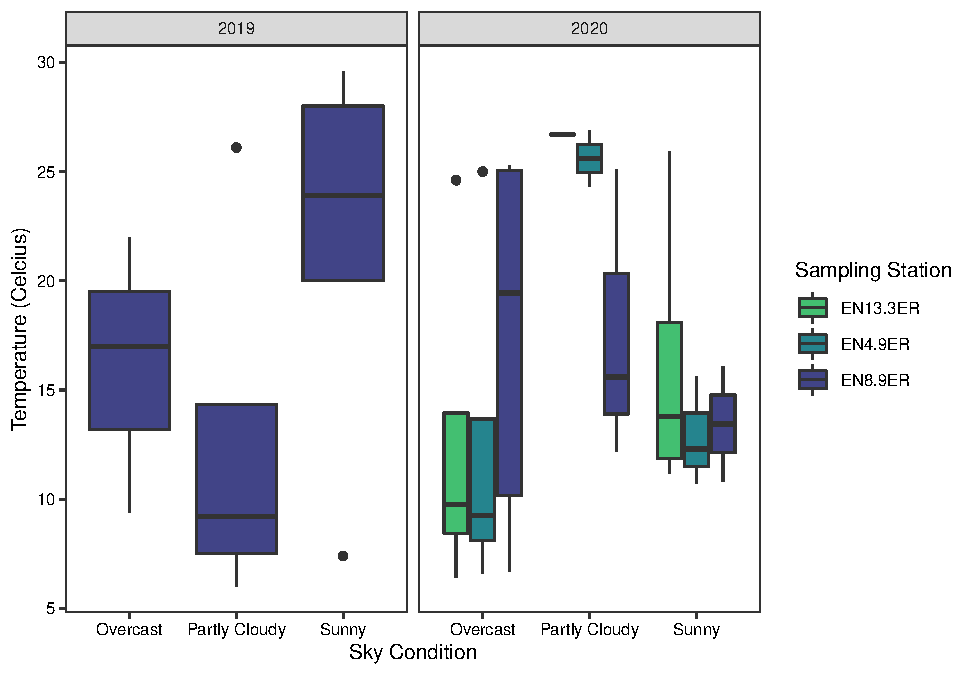
\includegraphics{August_Lindborg_ENV872_Project_files/figure-latex/unnamed-chunk-3-1.pdf}
\caption{Relationship between temperature and sky condition on each
sample day in Eno River for 2019 and 2020.}
\end{figure}

Additionally, as part of the explanatory analysis the relationship
between recent rainfall and turbidity was plotted. This relationship was
analyzed to determine the impact of rainfall on erosion in the Eno River
drainage area. Increased turbidity in the water following rain could be
an indicator that soil and other particles are enter the river through
erosion and surface runoff. The boxplot below shows relationship between
rain and turbidity for 2019 and 2020. There is only turbidity data for
one of the stations in 2019. However based on a visual comparison of the
plots, there appears to be much higher concentrations of turbidity when
is has rained in the last 24 hours. This relationship seems to be more
exaggerated in the 2020 data.

\begin{figure}
\centering
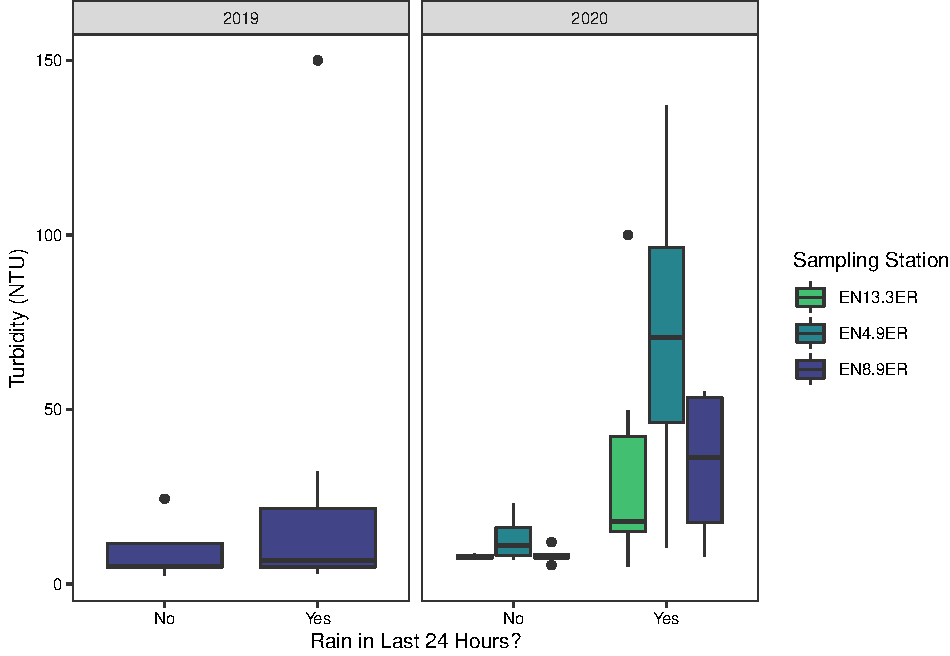
\includegraphics{August_Lindborg_ENV872_Project_files/figure-latex/unnamed-chunk-4-1.pdf}
\caption{Turbidity concentrations in Eno River for rain versus no rain
in the last 24 hours for 2019 and 2020.}
\end{figure}

In addition to assessing conditions at each of the monitoring sites, the
nine water quality parameters from 2019 and 2020 were visually compared.
First, 2019 and 2020 monthly dissolved oxygen concentrations were
plotted. Additionally, the North Carolina Water Quality Standard for
dissolved oxygen is included on the plot. Dissolved oxygen has a lower
limit standard of 4 ug/L. As shown below, concentrations of Dissolved
Oxygen follow similar trend across stations and across years. The
smoothed plot line shows that Dissolved Oxygen concentrations were
overall slightly higher in 2019 than in 2020. However, none of the
monthly dissolved oxygen concentrations fell below the lower limit of 4
ug/L.

\begin{figure}
\centering
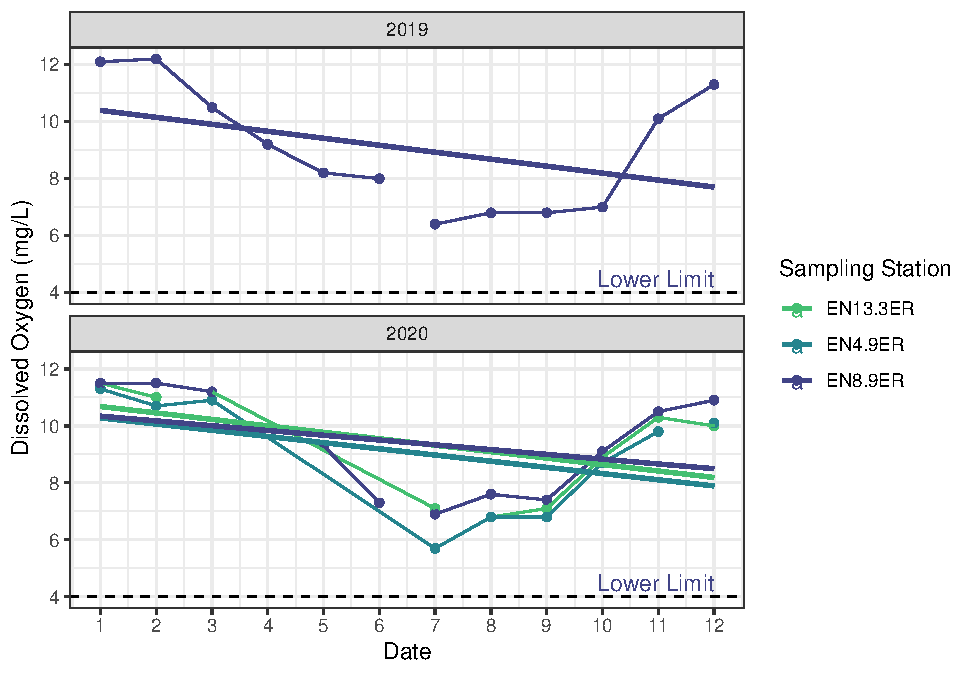
\includegraphics{August_Lindborg_ENV872_Project_files/figure-latex/unnamed-chunk-5-1.pdf}
\caption{Dissolved oxygen concentrations in 2019 and 2020 for Eno
River.}
\end{figure}

Visual comparisons of pH from 2019 and 2020, showed similar values
across stations and from 2019 to 2020. However, the maximum pH during
the Summer peak is high in 2019, \textasciitilde{} 7.5, than in 2020, 7.
Most of the pH data for both years shows that the pH in the Eno River is
within in the range permissible by North Carolina Water Quality
Parameters of 6-9. However, the December 2019 pH value is below the
lower limit of 6.

\begin{figure}
\centering
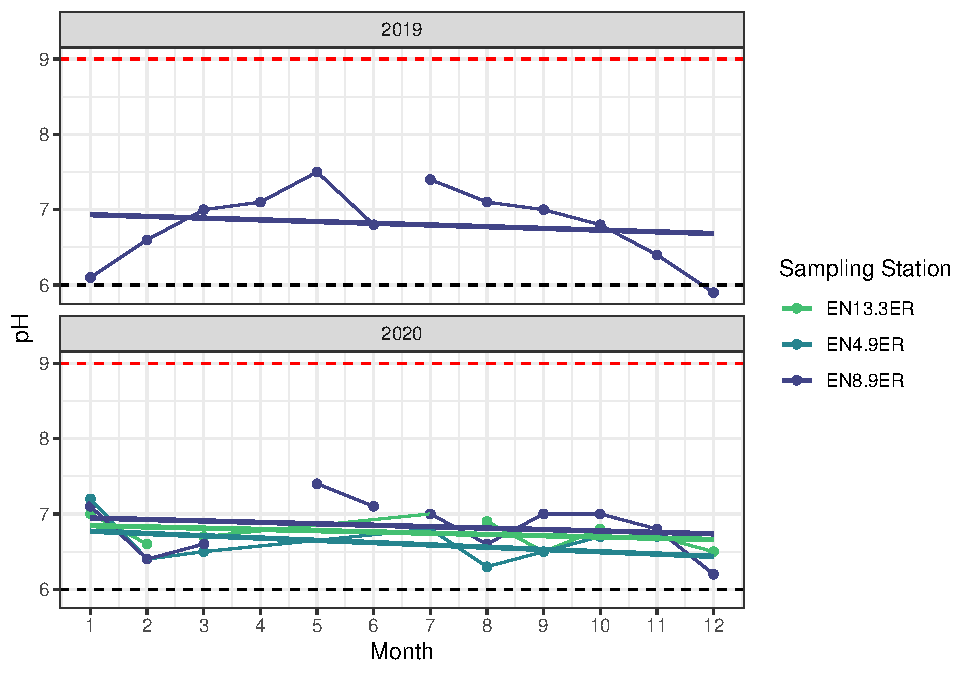
\includegraphics{August_Lindborg_ENV872_Project_files/figure-latex/unnamed-chunk-6-1.pdf}
\caption{pH in 2019 and 2020 for Eno River stations.}
\end{figure}

Based on the plots below, the Fecal Coliform has no discernible seasonal
trend in both the 2019 and 2020 graphs. Most of the measurements for
both years fall between 100 and 10,000. However, the maximum Fecal
Coliform concentrations in 2020 are much higher than 2019. The maximum
measured concentration in 2019 was approximately 5,000 and the maximum
measured concentration in 2020 was around 35,000. Additionally, the
North Carolina Water Quality Standard for fecal coliform is an upper
limit of 400 cfu/100mL, the concentrations of fecal coliform exceeds
this standard multiple time in 2019 and 2020.

\begin{figure}
\centering
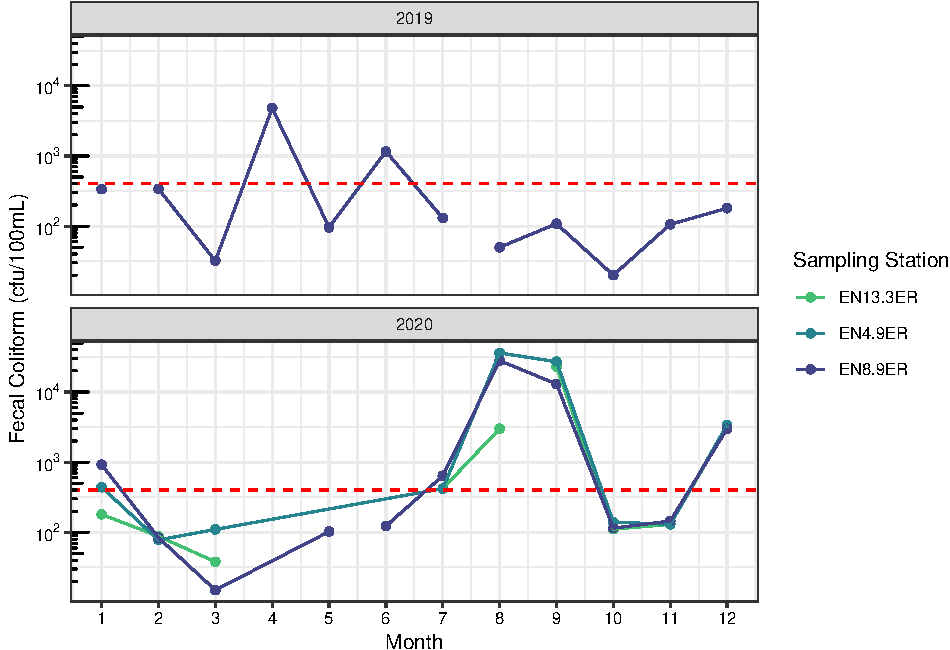
\includegraphics{August_Lindborg_ENV872_Project_files/figure-latex/unnamed-chunk-7-1.pdf}
\caption{Log-transformed fecal coliform in 2019 and 2020 for Eno River
stations.}
\end{figure}

The temperature data across stations and years shows a similar pattern
of maximum temperatures occurring in the late summer months. There
appears to be no significant difference in temperature between 2019 and
2020. Additionally, for both 2019 and 2020 the monthly temperatures are
below the standard of 32 degrees Celcius.

\begin{figure}
\centering
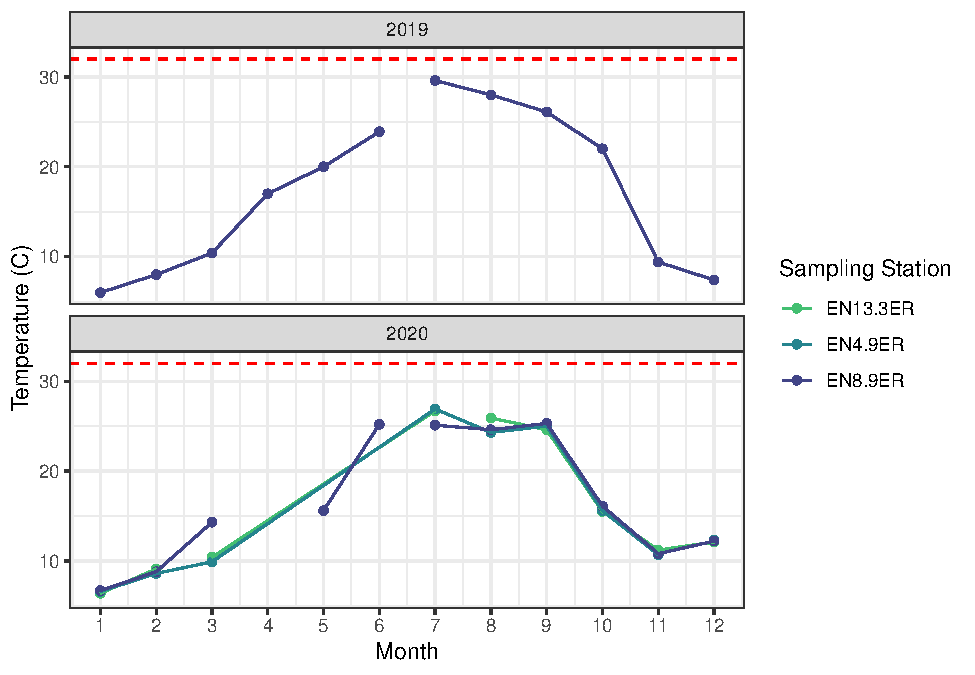
\includegraphics{August_Lindborg_ENV872_Project_files/figure-latex/unnamed-chunk-8-1.pdf}
\caption{Temperature in 2019 and 2020 for Eno River stations.}
\end{figure}

Based on the plotted data, total phosphorus has no discernible pattern
in the 2019 or 2020. Overall, concentrations seem relatively comparable
besides a greater maximum measured value in the 2019 data.

\begin{figure}
\centering
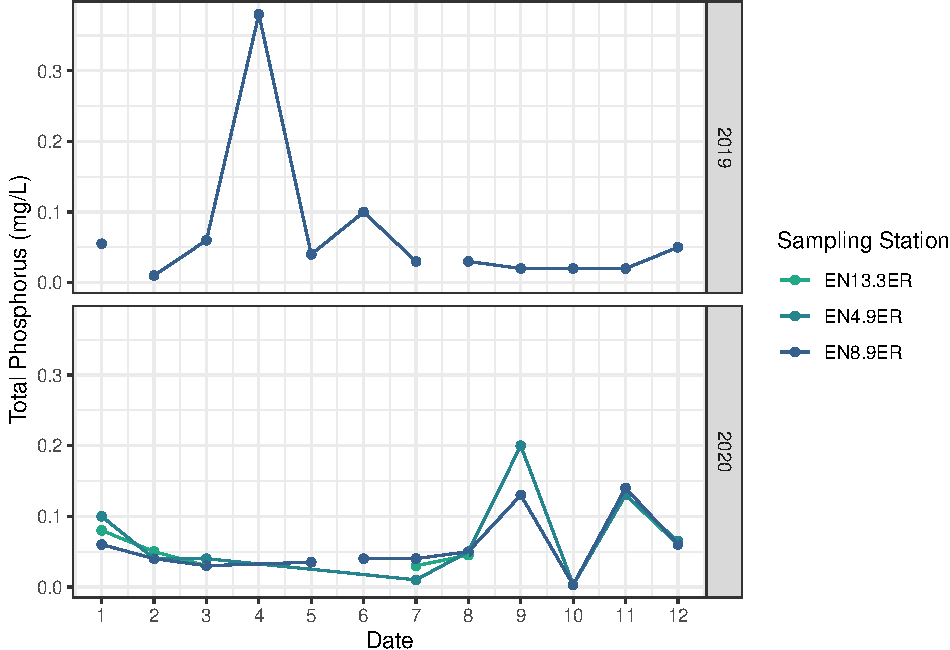
\includegraphics{August_Lindborg_ENV872_Project_files/figure-latex/unnamed-chunk-9-1.pdf}
\caption{Total phosphorus concentrations in 2019 and 2020 for Eno River
stations.}
\end{figure}

The plots of TSS show very different patterns across 2019 and 2020.
There are peaks in concentration in the Spring of 2019 and the late
Summer in 2020. Based on the plots, there appears to be greater TSS
measured in 2020 than 2019.

\begin{figure}
\centering
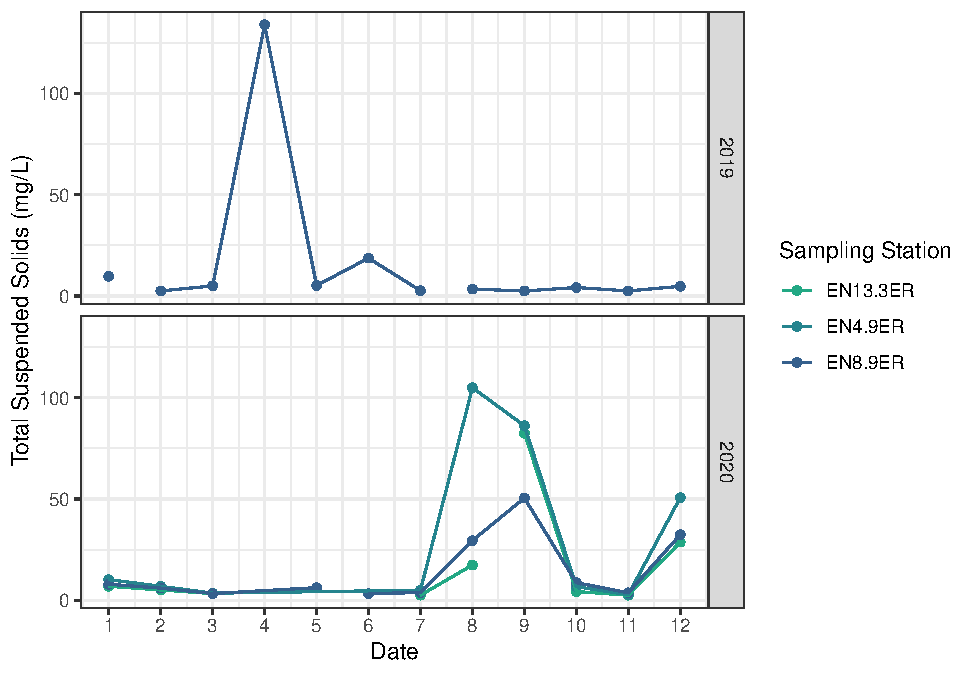
\includegraphics{August_Lindborg_ENV872_Project_files/figure-latex/unnamed-chunk-10-1.pdf}
\caption{Turbidity in 2019 and 2020 for Eno River stations.}
\end{figure}

The plots of turbidity show very different trends across 2019 and 2020.
Similar to TSS, there is a peak in the Spring of 2019 and the late
Summer of 2020. Based on the plots, the concentrations of Turbidity seem
to be higher in 2020. Additionally, there is one month in 2019 with a
Turbidity concentration above the North Carolina Water Quality Standard
of 50 NTU. In 2020, there were 3 months with turbidity above the 50 NTU
upper limit.

\begin{figure}
\centering
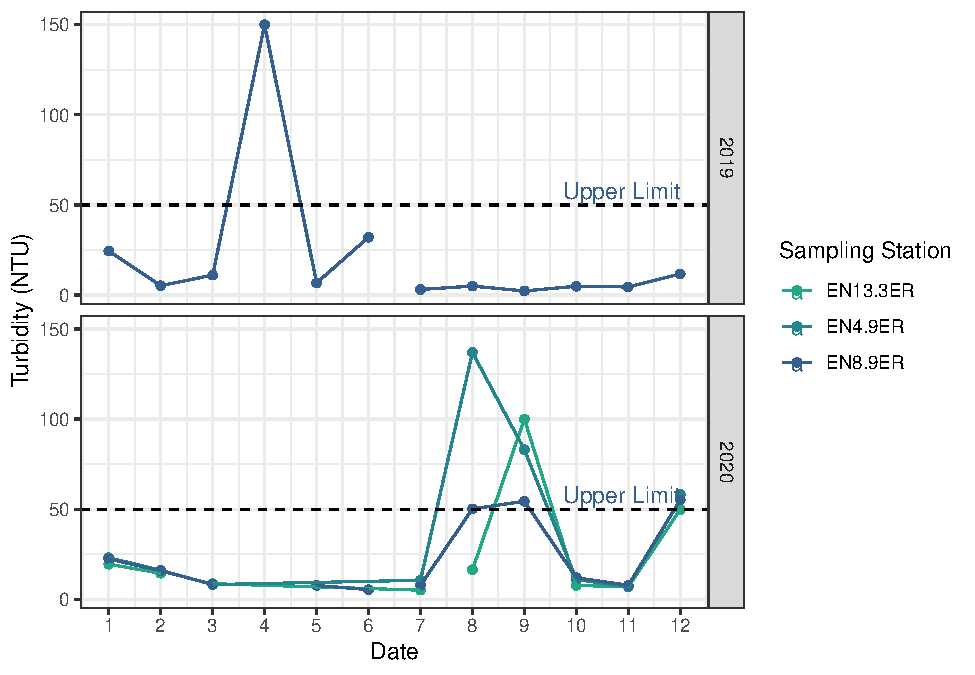
\includegraphics{August_Lindborg_ENV872_Project_files/figure-latex/unnamed-chunk-11-1.pdf}
\caption{Turbidity in 2019 and 2020 for Eno River stations.}
\end{figure}

Comparing the concentrations of Copper The Zinc concentrations are much
higher in 2019 than in 2020. This is expected based on the North
Carolina Water Quality Standards for each pollutant. Copper has an upper
concentration limit of 7 ug/L and Zinc has an upper limit of 50 ug/L.
Based on the plots, the Copper concentrations in Eno River appear
consistent between 2019 and 2020. However, the plot shows a significant
decrease in Zinc concentrations between 2019 and 2020. None of the
monthly concentrations of Copper or Zinc exceed the North Carolina Water
Quality Standards.

\begin{figure}
\centering
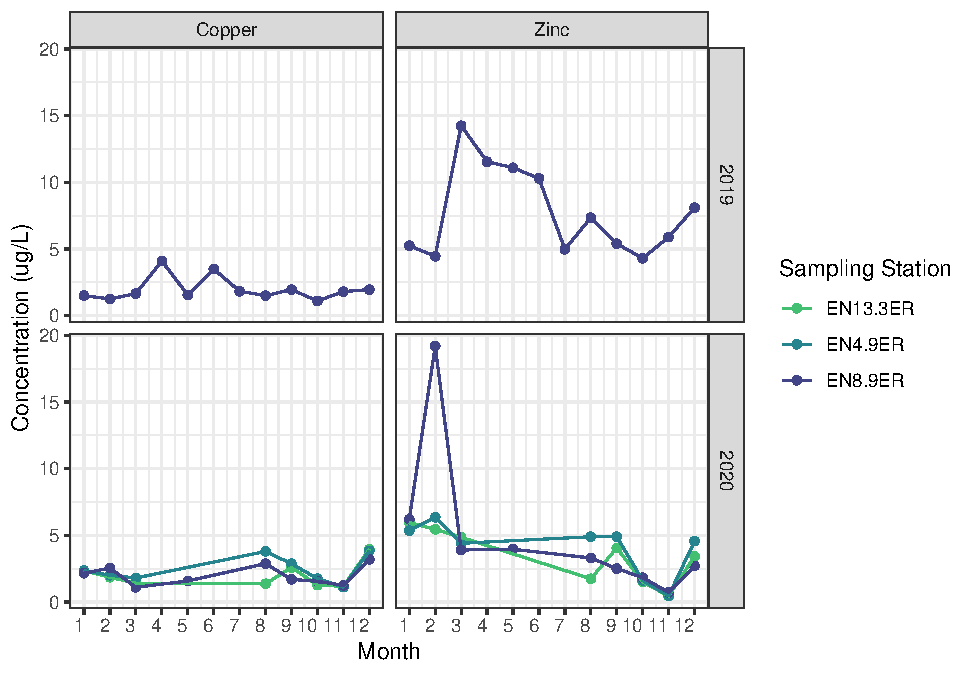
\includegraphics{August_Lindborg_ENV872_Project_files/figure-latex/unnamed-chunk-12-1.pdf}
\caption{Zinc and coppper concentrations in 2019 and 2020 for Eno River
stations.}
\end{figure}

\newpage

\hypertarget{ellerbe-creek}{%
\subsection{Ellerbe Creek}\label{ellerbe-creek}}

Visual explorations of the nine water quality parameters for Ellerbe
Creek were conducted to determine how these parameters changed between
2019 and 2020. First, because we are not able to visit the sites, we
wanted to determine what the main site characteristics may be. One main
exploration was the relationship between temperature and cloud cover,
hypothesizing that if temperature is fluctuating with changes in cloud
cover (e.g., temperatures increase on sunny days), this could indicated
minimal riparian vegetation. Minimal riparian vegetation has impacts on
water quality such as increased sedimentation, temperature, and runoff
contamination. At Ellerbe Creek, for all stations, it was observed that
temperature does not appear to change directly in response to cloud
cover (Figure 12). To make any definitive determinations about this
relationship, we would need more finite data than just one sample day
per month.

\begin{figure}
\centering
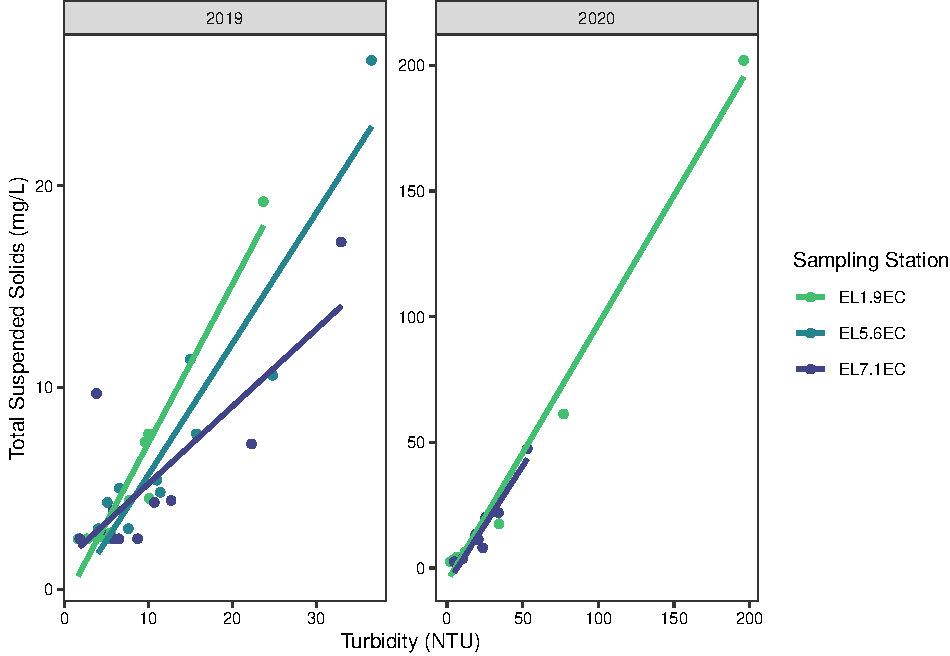
\includegraphics{August_Lindborg_ENV872_Project_files/figure-latex/unnamed-chunk-13-1.pdf}
\caption{Relationship between temperature and sky condition on sample
day in Ellerbe Creek for 2019 and 2020.}
\end{figure}

\newpage

We were also interested in the relationship between turbidity and rain,
as an indicator of erosion and to what degree the Ellerbe Creek sites
may be influenced by storm events. Visual comparisons show that there
appears to be an increase in turbidity after rain events, especially in
2020 (Figure 13). Figure 2 also reveals that there may be an increase in
turbidity between 2019 and 2020.

\begin{figure}
\centering
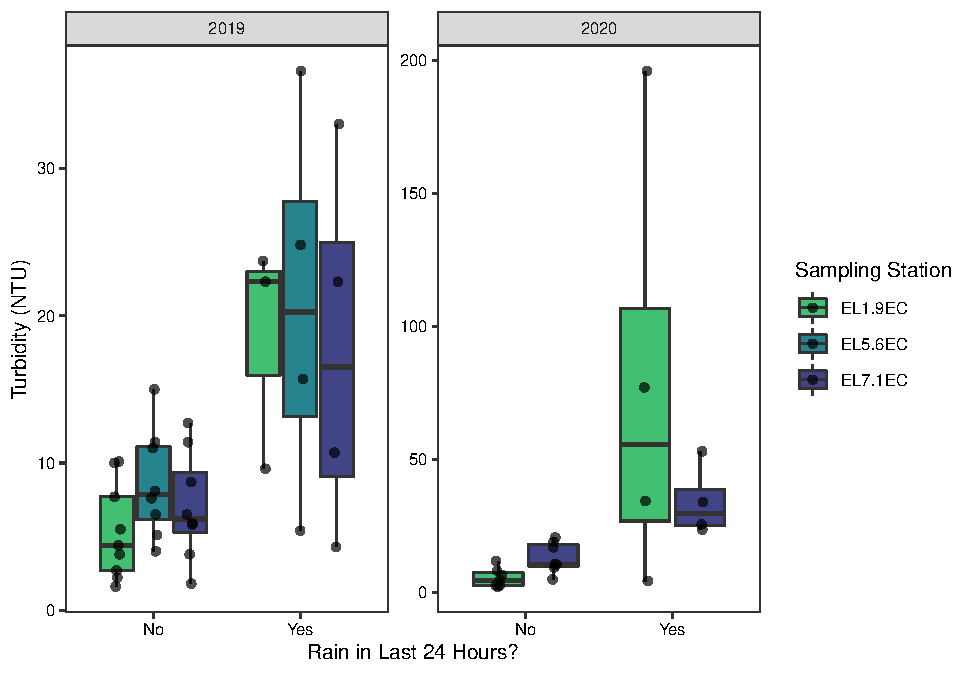
\includegraphics{August_Lindborg_ENV872_Project_files/figure-latex/unnamed-chunk-14-1.pdf}
\caption{Turbidity concentrations in Ellerbe Creek for rain versus no
rain in the last 24 hours for 2019 and 2020. Points represent samples
within each group.}
\end{figure}

After completing site explorations, we wanted to look specifically at
water quality parameters between 2019 and 2020. For dissolved oxygen,
there were no distinguishable trends over time and did not appear to be
differences between the sample sites for Ellerbe Creek (Figure 14).

\begin{figure}
\centering
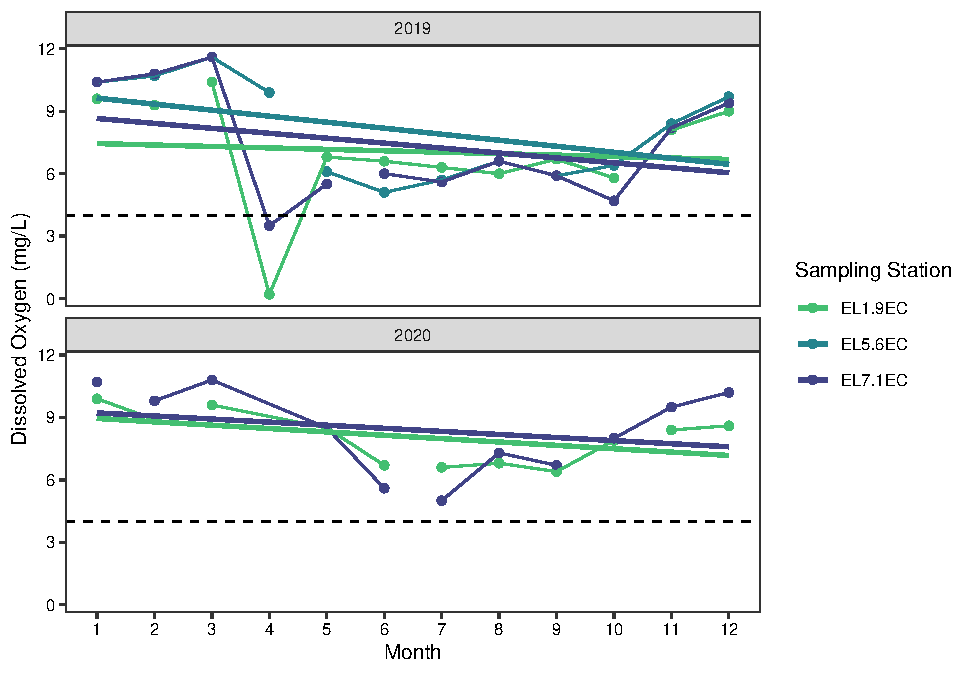
\includegraphics{August_Lindborg_ENV872_Project_files/figure-latex/unnamed-chunk-15-1.pdf}
\caption{Dissolved oxygen concentrations in 2019 and 2020 for Ellerbe
Creek stations. Black dashed line represents the lower limit water
quality standard for dissvoled oxygen.}
\end{figure}

There appeared to be downward trend in pH, particularly throughout the
year for 2020 (Figure 15), which warranted further investigation of this
parameter in the Analysis section.

\begin{figure}
\centering
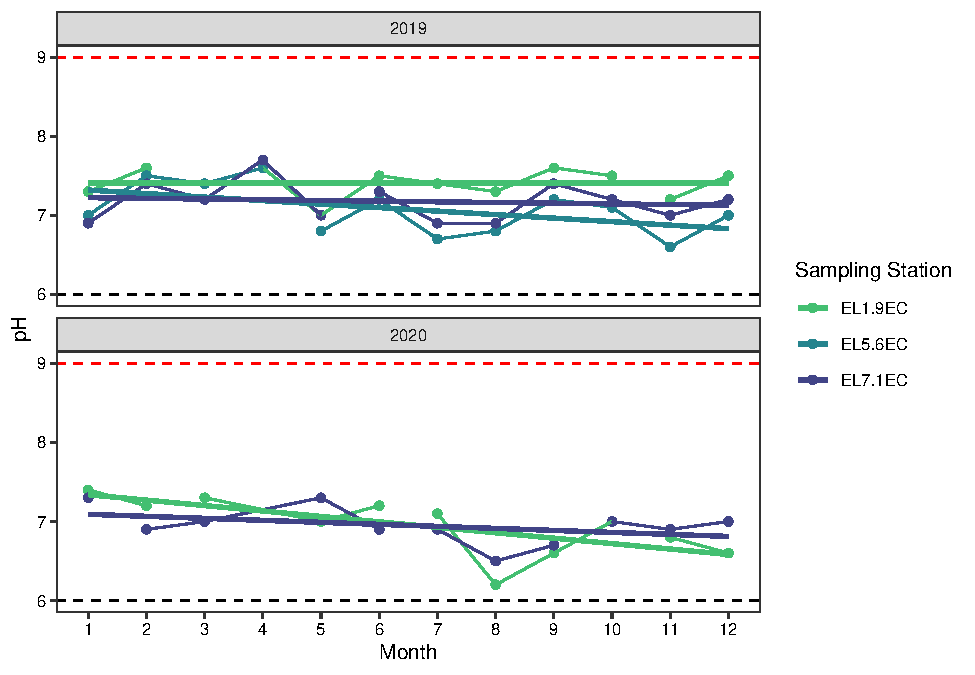
\includegraphics{August_Lindborg_ENV872_Project_files/figure-latex/unnamed-chunk-16-1.pdf}
\caption{pH in 2019 and 2020 for Ellerbe Creek stations. Black dashed
line represents the lower limit and red dashed line represents the upper
limit water quality standard for pH.}
\end{figure}

Fecal coliform was near the upper water quality limit for both years,
with spikes at both stations in August of both years greatly exceeding
the upper water quality limit of 400 cfu/100mL. There did not appear to
be a difference between the two years (Figure 16). Although we cannot
provide further analysis for the observed peaks, they could be
indicative of specific inputs to the creek around the same time each
year.

\begin{figure}
\centering
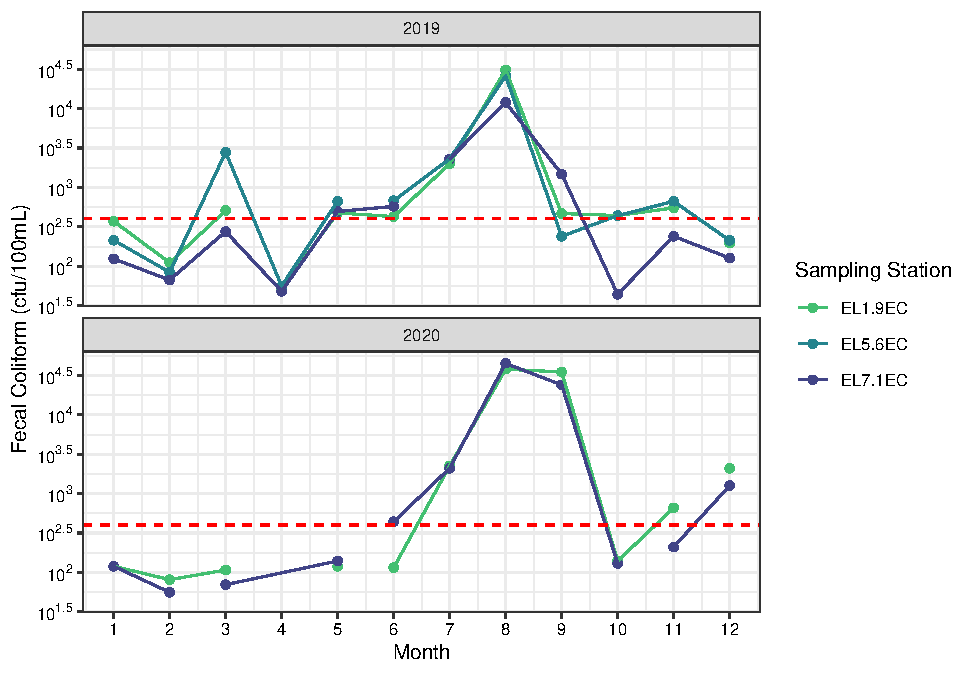
\includegraphics{August_Lindborg_ENV872_Project_files/figure-latex/unnamed-chunk-17-1.pdf}
\caption{Log-transformed fecal coliform in 2019 and 2020 for Ellerbe
Creek stations. Red dashed line represents the upper limit water quality
standard for fecal coliform.}
\end{figure}

Temperature was sporadic, which was expected based on seasonal
variations in ambient air temperature. Temperature fluctuations appeared
similar between both years and did not exceed maximum temperature
thresholds based on current water quality standards for streams of 32
degrees Celcius (Figure 17).

\begin{figure}
\centering
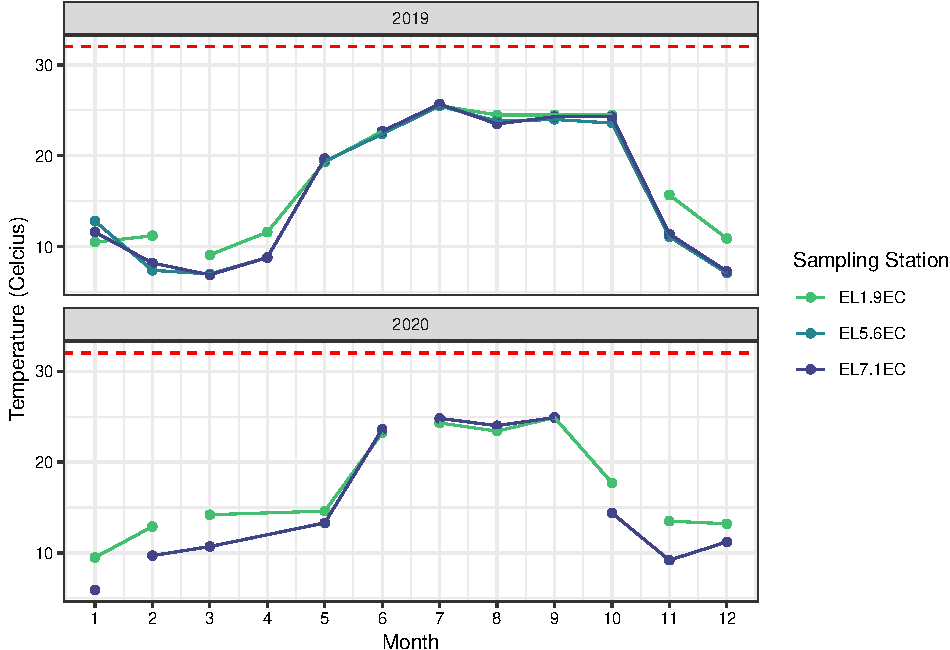
\includegraphics{August_Lindborg_ENV872_Project_files/figure-latex/unnamed-chunk-18-1.pdf}
\caption{Temperature in 2019 and 2020 for Ellerbe Creek stations. Red
dashed line represents the upper limit water quality standard for
temperature.}
\end{figure}

Total phosphorus appeared to increase throughout the year for both 2019
and 2020, but there did not appear to be an overall change in total
phosphorus between 2019 and 2020 (Figure 18). This is likely seasonal
due to temperature fluctuations and changing inputs throughout the year,
however there were not a sufficient number of data points to conduct
seasonal analyses.

\begin{figure}
\centering
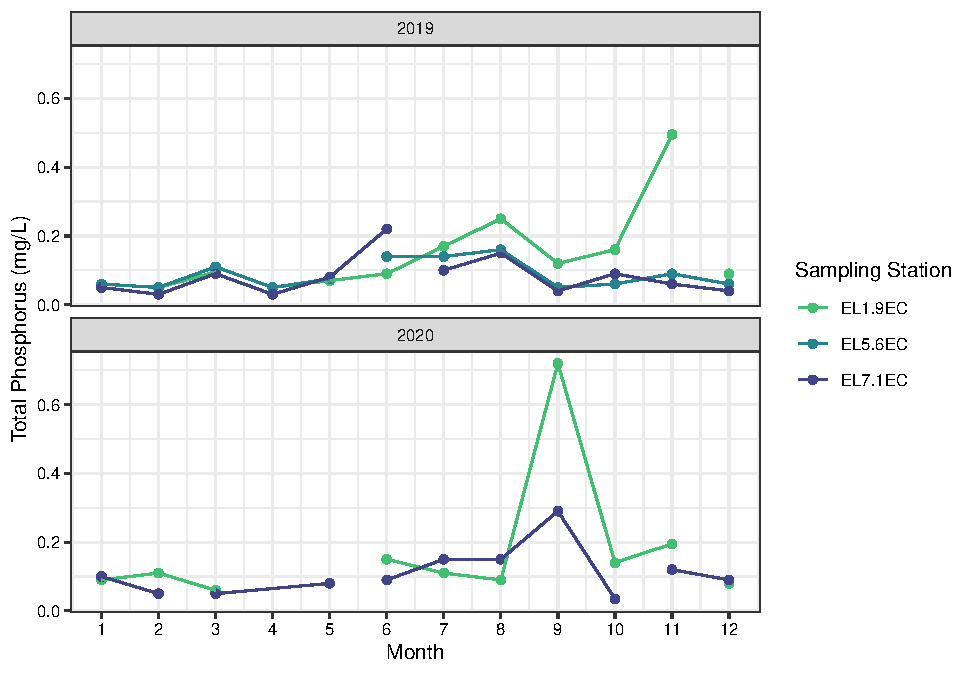
\includegraphics{August_Lindborg_ENV872_Project_files/figure-latex/unnamed-chunk-19-1.pdf}
\caption{Total phosphorus concentrations in 2019 and 2020 for Ellerbe
Creek stations.}
\end{figure}

Total suspended solids appeare to increase between 2019 and 2020, with
drastic spikes in concentrations during the late summer/early fall in
2020 for both sites that were not observed in 2019, when only a small
spike was observed (Figure 19). We were not able to provide further
analysis for why this peak was observed, but it could be due to input
changes around that time of year in 2020 compared to 2019.Further
analysis was conducted on the differences in TSS between 2019 and 2020
and is explained in the Analysis section.

\begin{figure}
\centering
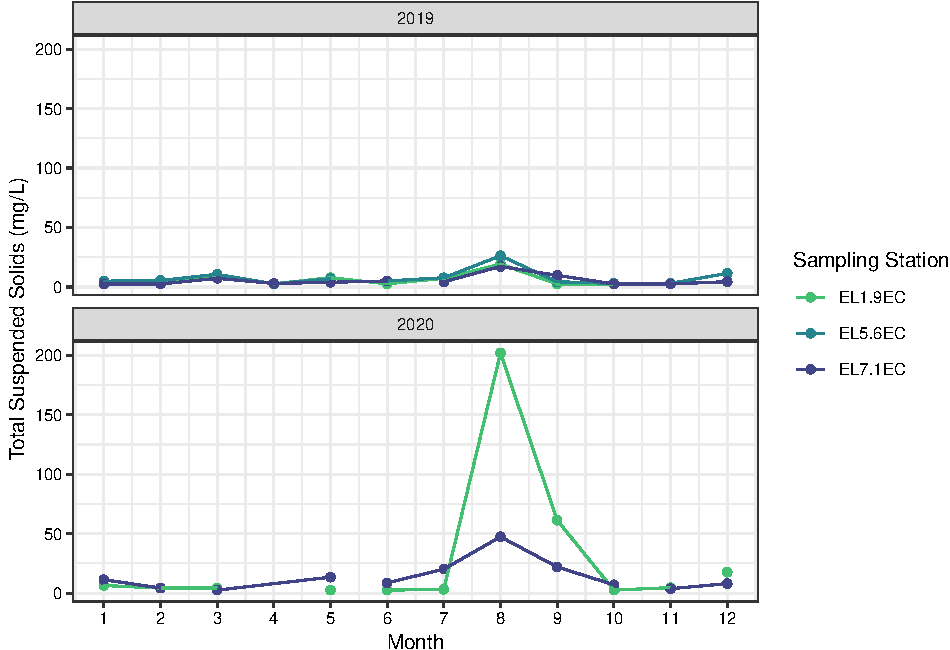
\includegraphics{August_Lindborg_ENV872_Project_files/figure-latex/unnamed-chunk-20-1.pdf}
\caption{Total suspended solids concentrations in 2019 and 2020 for
Ellerbe Creek stations.}
\end{figure}

Turbidity showed the same relationship as TSS, with values in 2020
appearing higher than those in 2019 and drastic peaks observed in late
summer/early fall. In 2019, values did not exceed the upper water
quality limit for turbidity. In 2020, values did exceed the upper limit
for site EL1.9EC in August and September and for site EL7.1EC in August
(Figure 20).

\begin{figure}
\centering
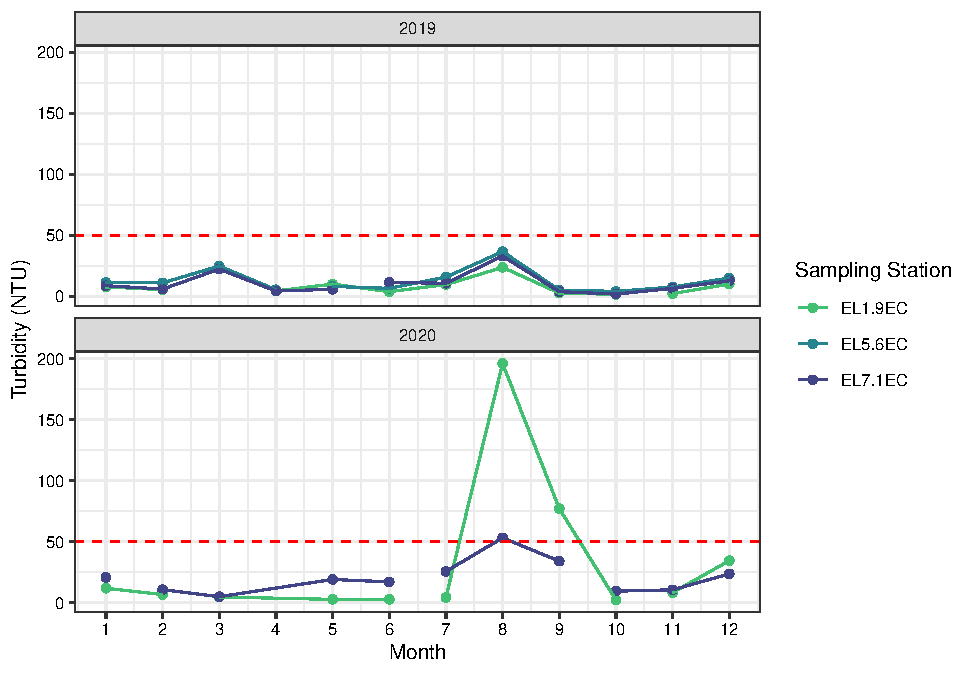
\includegraphics{August_Lindborg_ENV872_Project_files/figure-latex/unnamed-chunk-21-1.pdf}
\caption{Turbidity in 2019 and 2020 for Ellerbe Creek stations. Red
dashed line represents the upper limit water quality standard for
temperature.}
\end{figure}

Metal concentrations in Ellerbe Creek were below the water quality
standard for zinc and around or above the water quality standard for
copper. Zinc concentrations appeared to decrease while copper remained
consistent between 2019 and 2020 (Figure 21).

\begin{figure}
\centering
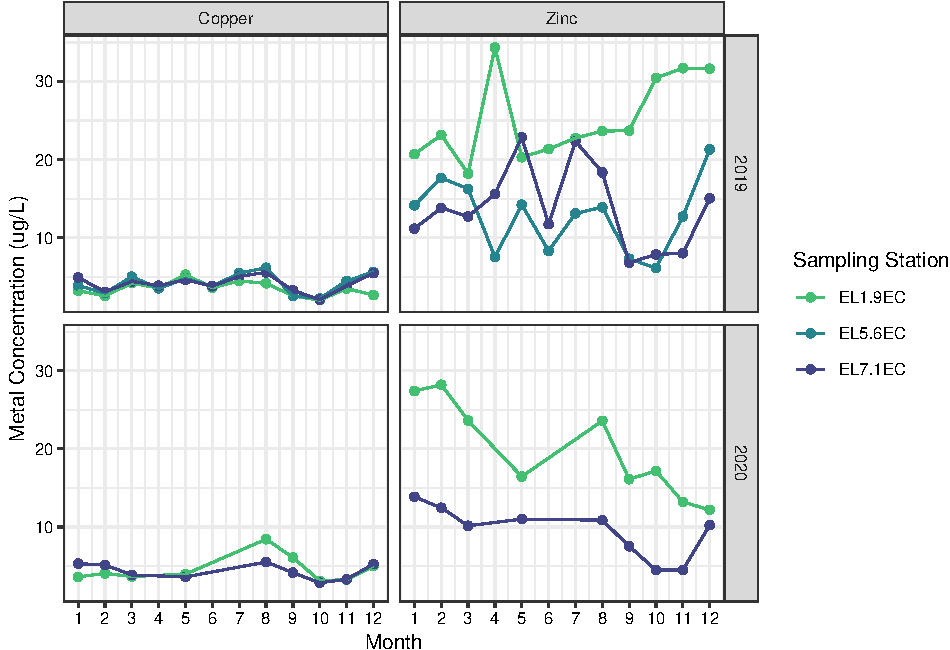
\includegraphics{August_Lindborg_ENV872_Project_files/figure-latex/unnamed-chunk-22-1.pdf}
\caption{Zinc and coppper concentrations in 2019 and 2020 for Ellerbe
Creek stations. Orange dashed line is the acute water quality standard
for copper and grey dashed line is the acute water quality standard for
Zinc in freshwater in North Carolina.}
\end{figure}

\newpage

\hypertarget{analysis}{%
\section{Analysis}\label{analysis}}

Based on the results of the exploratory analysis, certain parameters
were selected for additional analysis. Trends observed through visual
inspection of the exploratory analysis plots led to further analysis of
select water quality parameters.

\hypertarget{ph}{%
\subsection{pH}\label{ph}}

Exploratory analysis revealed that pH decreased slightly between 2019
and 2020 for both Ellerbe Creek and Eno River stations. An ANOVA was
conducted to determine the difference in pH between 2019 and 2020 across
all sites for each stream.

For Eno River, we performed an ANOVA which concluded that the difference
in pH from 2019 to 2020 is not statistically significant, (p-value =
0.54).

For Ellerbe Creek , pH was significantly lower in 2020 compared to 2019
(p-value \textless{} 0.01). However, mean pH for both years is within
what is considered the ``normal'' pH for streams (6-9), as shown by the
upper and lower limits in Figure 4.

The downward trend in Ellerbe Creek is concerning as it may cause pH
levels to dip below the lower limit in future years.

\hypertarget{zinc-copper}{%
\subsection{Zinc \& Copper}\label{zinc-copper}}

To determine whether there is a statistically significant change in
copper and zinc concentrations in the Eno River from 2019 to 2020. An
ANOVA was performed for 2019 and 2020 copper and zinc data. Based on the
p-value, the change in copper from 2019 to 2020 was found not to be
statistically significant (p-value = 0.6). However, the difference in
zinc concentrations from 2019 to 2020 was determined to be statistically
significant with a p-value \textless{} 0.01, with zinc concentrations
significantly lower in 2020.

An ANOVA conducted to determine the if concentrations differ for metals
between 2019 and 2020 in Ellerbe Creek revealed that there were no
statistical differences between 2019 and 2020 concentrations for mean
zinc (p-value = 0.22) or copper (p-value = 0.15) cocnentrations across
all sites combined.

\hypertarget{turbidity-and-recent-rainfall}{%
\subsection{Turbidity and Recent
Rainfall}\label{turbidity-and-recent-rainfall}}

Further analysis shows that the difference in turbidity in the Eno River
from rain within the last 24 hours was only statistically significant in
2020, with a p-value \textless{} 0.01. There are almost four times more
observations in 2020 than 2019 which may have impacted the ANOVA results
for 2019 since there were only 10 observations. Additionally, an ANOVA
of the Turbidity across years, showed that the difference in values from
2019 to 2020 was not statistically significant (p-value = 0.57).

In Ellerbe Creek, turbidity was significantly higher after rain event in
both 2019 and 2020 (p-values \textless{} 0.01), indicating that erosion
and sedimentation could be an issue for Ellerbe Creek. Additionally,
turbidity was significantly higher in 2020 compared to 2019 (p-value =
0.03).

\hypertarget{total-suspended-solids-tss-and-turbidity}{%
\subsection{Total Suspended Solids (TSS) and
Turbidity}\label{total-suspended-solids-tss-and-turbidity}}

The relationship between turbidity and TSS was conducted as a follow-up
analysis to determine if these measures are correlated. Typically, if
these values are correlated it indicates that observed turbidity and TSS
are the result of increased sediment and particulate matter, and not due
to other factors such as pollutants like dyes that impact one of these
measurements but not the other.

Figure 22 shows that TSS and Turbidity are closely linked and follow the
same trend across stations and across years in Eno River. These
parameters have similar peaks (see Exploratory Analysis figures). There
is some variation across stations, but the pattern remains the same
across. The results of the linear regression show that the two are
correlated (p-value \textless{} 0.01), and the R-squared value tells us
that 97\% of the variance in Total Suspended Solids can be explained by
variance in Turbidity.

The relationship between TSS and turbidity for Ellerbe Creek is shown in
Figure 23 and is similar to Eno River. Based on regression analysis,
these two values were correlated across all Ellerbe Creek sites combined
in 2019 (p-value \textless{} 0.01, R-squared = 0.76) and 2020 (p-value
\textless{} 0.01, R-squared = 0.98), again, indicating sedimentation is
an issue.

\begin{figure}
\centering
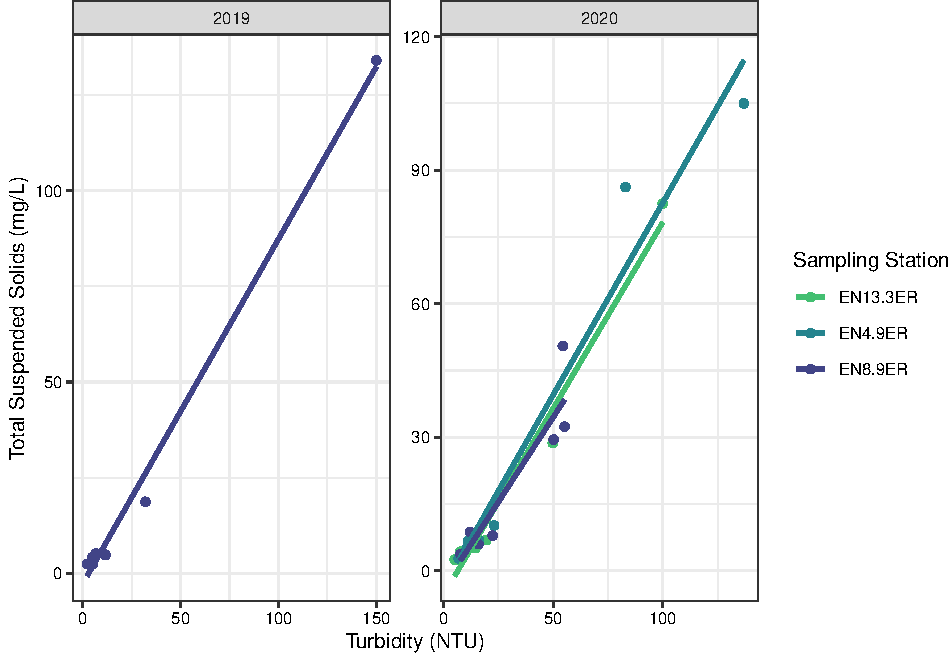
\includegraphics{August_Lindborg_ENV872_Project_files/figure-latex/unnamed-chunk-23-1.pdf}
\caption{Relationship between turbidity and total suspended solids for
all sites in Eno River in 2019 and 2020.}
\end{figure}

\begin{figure}
\centering
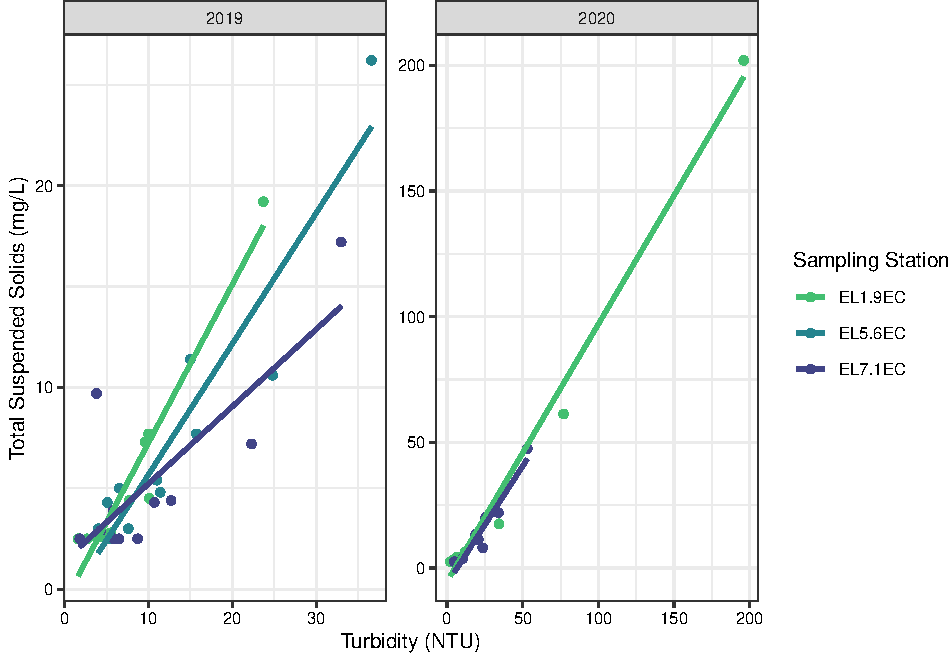
\includegraphics{August_Lindborg_ENV872_Project_files/figure-latex/unnamed-chunk-24-1.pdf}
\caption{Relationship between turbidity and total suspended solids for
all sites in Ellerbe Creek in 2019 and 2020.}
\end{figure}

\newpage

\hypertarget{summary-and-conclusions}{%
\section{Summary and Conclusions}\label{summary-and-conclusions}}

To assess the overall water quality of each stream, the NCDEQ Water
Quality Standards were referenced to identify exceedances in the
monitoring data across 2019 and 2020. In Eno River, pH fell below the
lower limit of 6 once in 2019. Additionally, fecal coliform
concentration in Eno River spiked above the upper limit of 400 cfu/100mL
for two months in 2019 and four months in 2020. Finally, the turbidity
in Eno River surpassed the water quality upper limit of 50 NTU once in
2019 and three times in 2020. Despite these exceedances,in Eno River the
nine water quality parameters assessed were within NCDEQ standards for
majority of 2019 and 2020. This signifies that overall Eno River is a
relatively healthy waterway that met a majority of the NCDEQ freshwater
quality standards in 2019 and 2020.

For exceedances in Ellerbe Creek, the dissolved oxygen concentration
fell below the NCDEQ lower limit of 4 mg/L for one month in 2019.
Additionally, the fecal coliform concentration in Ellerbe Creek exceeded
the upper limit of 400 cfu/100mL eight times in 2019 and six times in
2020. Also, the concentration of turbidity in Ellerbe Creek exceeded the
upper limit of 50 NTU, twice in 2020. Finally, the copper concentration
in Ellerbe exceeded the NCDEQ water quality standard of 7 ug/L once in
2020. Overall, Ellerbe Creek met a majority of the NCDEQ water quality
standards in 2019 and 2020 with the exception of fecal coliform which
had greater than 50\% exceedances. High bacteria in the water across
both years signifies the need for source control measures to identify
and abatement bacteria pollution. Based on the Ellerbe Creek Watershed
Management Improvement Plan, the City of Durham plans to address the
high bacteria in Ellerbe Creek through BMP implementation, stream
restoration projects, and sanitary sewer rehabilitation and replacement.

We suspected that water quality may show improvements in 2020 compared
to 2019, as some studies have shown that the COVID-19 pandemic has
resulted in improved surface water quality globally. Water quality
changes between 2019 and 2020 were variable for both Ellerbe Creek and
Eno River, with some parameters improving, most remaining the same, and
some getting worse. Zinc concentrations, for example, decreased in both
streams, but only significantly in Eno River. Turbidity on the other
hand increased in 2020 for both streams. Decrease in zinc concentrations
could be attributed to less road traffic. Break pads and tires release
metal particles, which are considered a major source of zinc in urban
streams. For turbidity, this could indicate more erosion and
sedimentation in 2020 compared to 2019. However, because rainfall and
turbidity are correlated, it could simply indicate that rainfall was
higher in 2020 compared to 2019, which we were not able to confirm. In
general, it appears that water quality did not improve overall from 2019
to 2020 in Eno River or Ellerbe Creek. It is interesting to note that
specific parameters did improve, such as zinc, likely as a result of
changes in urban traffic due to the pandemic.

Both streams met a majority of the NCDEQ water quality standards in 2019
and 2020. Eno River and Ellerbe Creek both had a number of exceedances,
but the majority of data for most parameters were within the NCDEQ
standards. However, fecal coliform concentration in Ellerbe Creek
exceeded the NCDEQ standard of 400 cfu/100mL for majority of the months
across 2019 and 2020. This signifies that Ellerbe Creek is an impaired
waterway with excessively and repetitively high bacteria concentrations.
Additionally, this trend was observed across both 2019 and 2020, which
supports the need for watershed improvements to address bacteria sources
in the Ellerbe Creek drainage area.

\newpage

\hypertarget{references}{%
\section{References}\label{references}}

City of Durham, Water Quality Data - Web Portal. (2021).
\url{http://www.durhamwaterquality.org/}

City of Durham. (2010, May). Ellerbe Creek Watershed Improvement Plan.
\url{https://durhamnc.gov/954/Ellerbe-Creek-Watershed-Improvement-Plan}

\end{document}
